% =========================================================================
% Physical Distributed GNSS Spoofing Evades Relative-Distance Detection
% in Compact UAV Swarms
% -------------------------------------------------------------------------
% Compile on Overleaf with pdfLaTeX + BibTeX.
% Figures are in figs/ ; bibliography in biblio.bib (style: IEEEtran).
% =========================================================================
\documentclass[conference]{IEEEtran}

\usepackage[utf8]{inputenc}
\usepackage[T1]{fontenc}
\usepackage{amsmath,amssymb}
\usepackage{graphicx}
\usepackage{booktabs}
\usepackage{multirow}
\usepackage{xcolor}
\usepackage[hidelinks]{hyperref}

\graphicspath{{figs/}}

\newtheorem{remark}{Remark}

\newcommand{\ptrue}[1]{\mathbf{p}_{#1}}
\newcommand{\pest}[1]{\hat{\mathbf{p}}_{#1}}
\newcommand{\PD}{P_{\mathrm{D}}}
\newcommand{\PFA}{P_{\mathrm{FA}}}
\newcommand{\todo}[1]{\textcolor{red}{\textbf{[TODO: #1]}}}

\begin{document}

\title{Physical Distributed GNSS Spoofing Evades\\
Relative-Distance Detection in Compact UAV Swarms}

\author{%
\IEEEauthorblockN{Silvia Schilleci}
\IEEEauthorblockA{\todo{affiliazione, email}}%
}

\maketitle

% =========================================================================
\begin{abstract}
Multi-receiver spoofing detection is regarded as one of the most robust
countermeasures against civilian GNSS spoofing: receivers in a known
formation compare the mutual distances implied by their GNSS fixes with
the formation geometry, and a single-transmitter spoofer---which forces
every victim onto the same position---is detected with near-certain
probability. We evaluate this detector family against a \emph{physical
distributed} spoofer: 24 fixed ground transmitters deployed around the
operating area of a 25-UAV swarm, each replaying the satellite closest
to it in azimuth, with capture decided by received power through an
elevation-dependent ground-to-UAV channel and with the replayed code
phase propagating over the true three-dimensional path to every drone.
No per-victim signal shaping and no idealized attack are simulated. We
implement the collapse detector of Jansen et al.\ (ACSAC~2016) in its
three variants and a two-sided formation-consistency test representative
of GNSS-vs-UWB checks for UAV swarms, and we evaluate them over the
5--20\,m inter-UAV spacing of outdoor GPS-based formation flight, with
20 Monte Carlo missions per configuration and bootstrap confidence
intervals. The attack displaces the swarm by 4\,km while the computed
formation is \emph{dilated} by about 23\,\% rather than collapsed, so
all three collapse detectors stay at $\PD\le0.011$ (95\,\% upper bound)
with ROC areas below chance (down to $0.001$) at every spacing. The
consistency test retains only marginal power, from $\PD=0.03$ at 5\,m to
$0.26$ at 20\,m at $\PFA=10^{-2}$, because the residual non-rigidity of
ground transmitters---caused by the mismatch between satellite and
transmitter elevations---is masked by GNSS noise at these spacings. We
derive the residual to first order, show that it depends critically on
deploying the array around the operating area, and delimit the result
with respect to direction-of-arrival and absolute-reference defenses.
\end{abstract}

\begin{IEEEkeywords}
GNSS spoofing, UAV swarms, spoofing detection, multi-receiver, distributed
attack, relative distances, formation flight.
\end{IEEEkeywords}

% =========================================================================
\section{Introduction}
\label{sec:intro}

Civilian GNSS signals carry no authentication: their structure and
navigation message are public, and a transmitter that reproduces them
with enough power can make a receiver compute any position and time of
the attacker's choosing. Since the first portable civilian spoofer was
demonstrated~\cite{humphreys2008assessing}, software-defined radios and
open-source signal generators have made the attack accessible for a few
hundred dollars, and incidents affecting ships, aircraft and unmanned
systems are now reported routinely~\cite{psiaki2016gnss}. Unmanned
aerial vehicles (UAVs) are a natural target: they navigate on GNSS by
default, and a swarm of UAVs flying in formation---for surveying,
inspection, delivery, or defense---multiplies both the value of the
target and the consequences of a successful hijack.

Among the many countermeasures proposed in the last fifteen
years~\cite{psiaki2016gnss,altaweel2023fanets}, \emph{multi-receiver}
detection stands out for its simplicity and for the strength of its
guarantee. Its principle, established by Tippenhauer et
al.~\cite{tippenhauer2011requirements}, is geometric: a spoofer with a
single antenna delivers the same set of signals to every receiver in its
coverage area, so all the victims compute the \emph{same} position fix.
A group of receivers that knows its own formation can therefore detect
the attack by checking that the mutual distances implied by the GNSS
fixes have not collapsed. Jansen et al.~\cite{jansen2016multireceiver}
turned this check into a calibrated statistical test, showing that four
receivers a few metres apart achieve a detection probability of $0.99$
at a false-alarm rate of $10^{-5}$; Swaszek and
Hartnett~\cite{swaszek2013multicots} derived its Neyman--Pearson optimal
form for commercial receivers. For UAV swarms the same idea has been
proposed with the formation measured on-line by inter-drone ultra-wideband
(UWB) ranging~\cite{mykytyn2023uwb} or verified as a localization
feasibility problem~\cite{bi2024sdp}. The guarantee rests on one
assumption: that the attacker has a single transmission point.

This paper asks what happens when that assumption is dropped in the most
concrete way possible---not with an idealized attacker that imposes a
common offset on every victim, but with a \emph{physical distributed}
spoofer made of several fixed ground transmitters surrounding the
swarm's operating area, each impersonating one satellite, subject to
real propagation geometry and to a realistic ground-to-UAV channel. Such
an attacker is within reach of a well-resourced adversary (two dozen
synchronized software-defined radios), and recent work has shown
formation-preserving spoofing to be feasible in hardware when the
transmitters are placed along the satellite directions at
altitude~\cite{tibaldo2025gnsswasp}. Ground-based transmitters, however,
cannot reproduce the satellites' elevation, and the question of how much
of the single-transmitter detection guarantee survives against them has
not been quantified.

We answer it by simulation, for the inter-UAV spacing of 5 to 20\,m that
characterizes outdoor GPS-based formation flight (Section~\ref{sec:setup}).
Our contributions are:
\begin{itemize}
\item a transmitter-by-transmitter simulation model of a distributed
  ground spoofer attacking a moving UAV swarm, with per-epoch routing of
  satellites to transmitters, true three-dimensional propagation of the
  replayed signals, and the elevation-dependent ground-to-UAV path-loss
  model of~\cite{alhourani2018cellular} (Section~\ref{sec:attack});
\item a faithful implementation of the collapse detector
  of~\cite{jansen2016multireceiver} in its three variants, and of a
  two-sided formation-consistency test representative of GNSS-vs-ranging
  checks~\cite{mykytyn2023uwb,stenberg2022multiple}
  (Section~\ref{sec:detection});
\item a Monte Carlo evaluation with mission-level bootstrap confidence
  intervals showing that the physical attack displaces the swarm by
  kilometres while \emph{dilating}, not collapsing, the computed
  formation: the collapse detectors are driven below chance at every
  spacing, and the consistency test retains only marginal power
  ($\PD\le0.26$ at $\PFA=10^{-2}$) (Section~\ref{sec:results});
\item a first-order analysis of the residual non-rigidity of a ground
  array, which identifies the satellite-vs-transmitter elevation mismatch
  as its cause, shows its dependence on the array deployment, and
  delimits the result with respect to direction-of-arrival and
  absolute-reference defenses (Sections~\ref{sec:residual}
  and~\ref{sec:discussion}).
\end{itemize}
The simulator and the detection code are released with the paper.

% =========================================================================
\section{Related Work}
\label{sec:related}

\subsection{Multi-receiver detection in the position domain}
Tippenhauer et al.~\cite{tippenhauer2011requirements} formalized the
GPS group-spoofing problem and proved two complementary results: a
single-antenna spoofer places all victims at the same location
(Result~1), and a formation-preserving placement of one transmitter per
impersonated satellite always exists, along the satellite directions
(Result~7). Their countermeasure checks that the computed positions
preserve the physical formation, without a statistical model. Jansen et
al.~\cite{jansen2016multireceiver} supplied the model: the pairwise
distances between receivers are Rician under authentic conditions and
Rayleigh under a single-transmitter attack, with spatially correlated
position noise ($\sigma\approx0.5$--$3$\,m, $\rho\approx0.4$--$0.6$
measured), and the test $f(\{d_{ij}\})<\lambda$ is evaluated in minimal,
maximal, majority and normalized-majority variants, the last being the
best. Their prototype with four receivers on a 5\,m square ran for three
hours without errors; their own attempt at a distance-preserving
four-USRP attack succeeded on one receiver and failed on two. Swaszek
and Hartnett~\cite{swaszek2013multicots} derived Neyman--Pearson optimal
tests for COTS receivers at known relative positions, and later fused
GNSS fixes with inter-vehicle ranges for platoons under the assumption
that only one vehicle is spoofed~\cite{swaszek2017platoon}.
Crowd-GPS-Sec~\cite{jansen2018crowdgpssec} applies the collapse
principle to crowdsourced air-traffic receivers, combined with an
absolute time-difference-of-arrival reference.

\subsection{Measurement-domain and swarm variants}
In the measurement domain, Stenberg et al.~\cite{stenberg2022multiple}
test double differences of pseudorange and carrier phase between
receivers with a $\chi^2$ GLRT, finding a minimum receiver separation of
about 5\,m with standard positioning; Kalantari and
Larsson~\cite{kalantari2020rigidbody} derive a GLRT for receivers on a
rigid body with unknown pose explicitly against multiple spoofers,
showing that more receivers make the attack harder; Borio and
Gioia~\cite{borio2016sumofsquares} detect the single common direction of
arrival with a two-receiver carrier-phase sum-of-squares statistic. For
UAV swarms, Mykytyn et al.~\cite{mykytyn2023uwb} compare GNSS-derived
inter-drone distances with UWB two-way ranging and raise an alarm when
they differ by more than about 5\,m, dismissing a coordinated per-drone
attack as "virtually impossible"; Bi et al.~\cite{bi2024sdp} cast
detection as a semidefinite localization-feasibility problem robust to
colluding members. GNSS/INS fusion defenses such as
SemperFi~\cite{sathaye2022semperfi} and tightly coupled INS innovation
monitors~\cite{tanil2018insmonitor,kujur2024insmonitor} compare the GNSS
track with inertial dead reckoning and respond to the time variation of
the induced error.

\subsection{Coordinated and distributed spoofing}
Attack-side work has progressively approached the formation-preserving
placement of~\cite{tippenhauer2011requirements}. Ceccato et
al.~\cite{ceccato2020spatial} designed a multi-antenna ground spoofer
with Wiener precoding that displaces a swarm without disrupting its
formation, at the level of a mathematical model; Chen et
al.~\cite{chen2025swarmspoofing} analyze formation-preserving spoofing of
small swarms with software-defined radios;
GNSS-WASP~\cite{tibaldo2025gnsswasp} demonstrated in hardware a
constellation of at least four GPSDO-synchronized transmitters, placed
in line with the satellites at altitude, that spoofs an arbitrary number
of receivers over a square kilometre while preserving their relative
distances to within a metre, explicitly bypassing
multi-receiver~\cite{jansen2016multireceiver} and
sensor-fusion~\cite{sathaye2022semperfi} countermeasures. Park and
Yoo~\cite{park2026rigidshift} state the translation-invariance of
relative-only detectors as a formal proposition, rooted in the gauge
freedom of anchor-free network
localization~\cite{aspnes2006localization}, and evaluate it by
simulation with an idealized common offset. Surveys of UAV spoofing
defenses~\cite{altaweel2023fanets,sebastian2026survey} note that
detectors relying on neighbours' positions fail when the neighbours are
inside the spoofed area, but none quantifies the effect for a physical
ground array.

\subsection{Positioning of this work}
Our attacker is deliberately more constrained than those
of~\cite{tibaldo2025gnsswasp,park2026rigidshift}: fixed transmitters on
the ground, no per-victim adaptation, a measured channel. The quantity we
report is precisely what separates it from the ideal formation-preserving
attack---the residual deformation of the computed formation---and its
consequence for the two families of relative-distance detectors over the
spacing range of real formation flight.

% =========================================================================
\section{System Model}
\label{sec:system}

\subsection{Swarm, constellation, and measurement model}
We consider a swarm of $m=25$ UAVs flying in a square $5\times5$ grid
with spacing $g$ (the \emph{formation spacing}), following a way-point
trajectory at altitudes between 100 and 700\,m that spans about 7\,km
around its start point; positions are sampled every $T_s=5$\,s over a
20-minute mission. The GNSS constellation is modeled as
$N_{\mathrm{sat}}=24$ satellites on 6 circular orbital planes
(inclination $55^\circ$, altitude 20\,200\,km) over a rotating spherical
Earth. For UAV $u$ at position $\ptrue{u}(t)$ and satellite $s$ at
position $\mathbf{s}_s(t)$ (visible when its elevation is positive), the
authentic propagation delay is
$\tau_{u,s}(t)=\lVert\mathbf{s}_s(t)-\ptrue{u}(t)\rVert/c$. Each receiver
has a clock bias $\delta t_u\sim\mathcal{U}(-1,1)$\,s, constant over the
mission, and each pseudorange carries additive white Gaussian noise of
standard deviation $\sigma_{\mathrm{pr}}=3$\,m, representative of
standard (non-differential) positioning.

Each UAV computes its position fix $\pest{u}$ independently by iterated
linearized least squares (Gauss--Newton) over the four unknowns
$(x,y,z,\delta t)$: at iteration $k$, with predicted ranges
$R_s=\lVert\mathbf{s}_s-\hat{\mathbf{x}}^{(k)}\rVert$ and pseudoranges
$\rho_s=c\,(\tilde{\tau}_{u,s}-\widehat{\delta t}^{(k)})$,
\begin{equation}
\mathbf{G}\,\Delta =\boldsymbol{\rho}-\mathbf{R},\qquad
\mathbf{G}_{s,:}=\Bigl[\tfrac{(\hat{\mathbf{x}}-\mathbf{s}_s)^{\!\top}}{R_s},\; c\Bigr],
\label{eq:ls}
\end{equation}
solved in the least-squares sense for five iterations, where
$\tilde{\tau}_{u,s}$ is the \emph{measured} delay (authentic or spoofed).
Without attack and noise the solver returns the true grid positions to
numerical precision (error $<10^{-4}$\,m), so estimated and true
positions are expressed in the same frame.

In addition to GNSS, the UAVs measure their instantaneous mutual
distances with an independent on-board ranging sensor (UWB two-way
ranging, as in~\cite{mykytyn2023uwb}):
\begin{equation}
d^{\mathrm{meas}}_{ij}(t) = \lVert\ptrue{i}(t)-\ptrue{j}(t)\rVert
 + \varepsilon_{ij}(t),\quad
\varepsilon_{ij}\sim\mathcal{N}(0,\sigma^2_{\mathrm{rng}}),
\label{eq:uwb}
\end{equation}
with $\sigma_{\mathrm{rng}}=0.1$\,m. This is the most favorable setting
for the defender: the true formation is known essentially without error
at every epoch.

\subsection{Ground-to-UAV channel}
Spoofing signals travel over a ground-to-air link. We adopt the
suburban cellular-to-UAV path-loss model of Al-Hourani and
Gomez~\cite{alhourani2018cellular}: for a ground transmitter at
horizontal distance $d$ and elevation angle $\theta$ (in degrees) as seen
from the UAV,
\begin{equation}
\mathrm{PL}(d,\theta) = 10\,\alpha\log_{10}(d)
 + A\,(\theta-\theta_0)\,e^{-\frac{\theta-\theta_0}{B}} + \eta_0
 \quad [\mathrm{dB}],
\label{eq:alhourani}
\end{equation}
with $\alpha=3.04$, $A=-23.29$, $B=4.14$, $\theta_0=-3.61^\circ$,
$\eta_0=20.70$\,dB (shadowing disabled for repeatability). The
excess-loss term is fitted in~\cite{alhourani2018cellular} for
$\theta\in[-2^\circ,10^\circ]$ and is saturated at $10^\circ$ beyond;
with the deployment of Section~\ref{sec:attack} no link exceeded this
limit in any run, so the model is always used within its validity range.
Authentic signals follow free-space loss from satellite transmit power
$P_t^{\mathrm{sat}}=25$\,W with antenna gains
$G_t^{\mathrm{sat}}=13.5$\,dB and $G_r=5$\,dB, giving received powers
of about $-150$\,dBW.

% =========================================================================
\section{Physical Distributed Spoofing Attack}
\label{sec:attack}

The attacker's goal is to displace the whole swarm's perceived position
onto a decoy point about 5.7~km from the flight path, while the swarm
believes it is following its mission plan. The attack is simulated
transmitter by transmitter; nothing is assumed about per-victim signal
shaping.

\subsection{Transmitter geometry and per-epoch routing}
$N_{\mathrm{sp}}=24$ fixed ground transmitters are placed on a circle of
radius $R_{\mathrm{sp}}=10$\,km enclosing the swarm's operating area
(Fig.~\ref{fig:scenario}), each radiating $P_t^{\mathrm{sp}}=1$\,mW with
$G_t^{\mathrm{sp}}=1$\,dB. Following the geometric argument
of~\cite[Result~7]{tippenhauer2011requirements}, each visible satellite
$s$ is routed, at every epoch, to the transmitter whose azimuth as seen
from the \emph{current} true swarm centre $\mathbf{p}^{\mathrm{ctr}}(t)$
is closest to the satellite's azimuth:
\begin{equation}
\mathrm{sp}(s,t)=\arg\min_{k}\;
\bigl|\angle_{2\pi}\bigl(\phi_s(t)-\phi_k(t)\bigr)\bigr| .
\label{eq:assign}
\end{equation}
The transmitters never move; only the routing is updated, which requires
the attacker to track the swarm centre---the same knowledge it needs to
calibrate the replayed delays.

\subsection{Capture and replayed delay}
For each UAV $u$ and visible satellite $s$ the receiver locks onto the
transmitter whenever the received spoofing power, computed
with~\eqref{eq:alhourani}, exceeds the authentic one. With the chosen
EIRP the spoofer margin over the satellite is between 13 and 29\,dB on
every link (median 19.5\,dB), so capture is complete and homogeneous
across the swarm: no UAV mixes authentic and spoofed satellites.

Transmitter $k=\mathrm{sp}(s,t)$ replays the signal of satellite $s$ with
its code phase calibrated so that, at the true swarm centre, the measured
delay equals the decoy delay $\tau^{\mathrm{dec}}_{s}$---the delay that
satellite $s$ would exhibit at the decoy position. A UAV at a different
position receives the same transmission over a different path and
measures
\begin{equation}
\tilde{\tau}_{u,s} \;=\; \tau^{\mathrm{dec}}_{s}\;-\;\delta t_u\;+\;
\frac{\lVert\mathbf{q}_k-\ptrue{u}\rVert-\lVert\mathbf{q}_k-\mathbf{p}^{\mathrm{ctr}}\rVert}{c},
\label{eq:power}
\end{equation}
where $\mathbf{q}_k$ is the transmitter position and both norms are true
three-dimensional slant distances. The last term is the physical
propagation residual: it vanishes for the centre UAV, which computes
exactly the decoy position, and is nonzero for the other UAVs.

\subsection{Residual non-rigidity of a ground array}
\label{sec:residual}
Write $\ptrue{u}=\mathbf{p}^{\mathrm{ctr}}+\boldsymbol{\delta}_u$ with
$\lVert\boldsymbol{\delta}_u\rVert\ll\lVert\mathbf{q}_k-\mathbf{p}^{\mathrm{ctr}}\rVert$.
To first order the residual in~\eqref{eq:power} is
$-(\hat{\mathbf{w}}_k\!\cdot\!\boldsymbol{\delta}_u)/c$, with
$\hat{\mathbf{w}}_k$ the unit vector from the centre to the transmitter,
whereas the delay that would make UAV $u$ compute the decoy position
\emph{rigidly displaced} by $\boldsymbol{\delta}_u$ is
$-(\hat{\mathbf{e}}_s\!\cdot\!\boldsymbol{\delta}_u)/c$, with
$\hat{\mathbf{e}}_s$ the unit line of sight to the satellite. For a
horizontal swarm and azimuth-matched routing the per-satellite
pseudorange error is
\begin{equation}
\epsilon_{u,s}\;\approx\;
(\hat{\mathbf{a}}_s\!\cdot\!\boldsymbol{\delta}_u)\,
\bigl(\cos\theta_k-\cos\mathrm{el}_s\bigr),
\label{eq:residual}
\end{equation}
where $\hat{\mathbf{a}}_s$ is the satellite azimuth direction, $\theta_k$
the near-zero elevation of the ground transmitter and $\mathrm{el}_s$ the
satellite elevation. A ground transmitter cannot reproduce the
satellite's elevation, so~\eqref{eq:residual} vanishes only for
satellites near the horizon. Its coefficient is positive for every
satellite: a UAV displaced \emph{towards} satellite $s$ measures a
pseudorange longer than the rigid one, so the least-squares solver places
it farther from the centre than it is. The error scales with the
baseline and the computed formation is therefore \emph{dilated}---a
systematic outward displacement of every UAV, modulated by the
elevations of the satellites in view---rather than collapsed.
Section~\ref{sec:results} measures the dilation at about 23\,\% of the
baseline.

Two further facts, established numerically, matter for an attacker. The
residual does not depend on transmitter power: capture is already
complete at 1\,mW and raising the power to 10\,W leaves the deformation
unchanged. It depends critically on the array enclosing the operating
area: with a 2.5\,km array centred on the start point the swarm is
inside the circle only 26\,\% of the time, and the deformation grows
from 12\,\% inside to 55\,\% outside (correlation $0.98$ with the
distance from the array centre), because from outside the array all
transmitters lie in a narrow angular sector and no routing can match the
satellite azimuths.

\begin{remark}[Why collapse detectors are blind]
\label{rem:collapse}
The collapse detectors of Section~\ref{sec:detection} threshold a
statistic that decreases when the pairwise distances shrink---the
signature of a single transmitter seen by all
receivers~\cite[Result~1]{tippenhauer2011requirements}. A distributed
spoofer with one transmitter per satellite delivers to every UAV a
different set of delays, consistent to first order with its own
displacement from the centre, and the residual~\eqref{eq:residual}
dilates the formation. The statistic therefore moves \emph{away} from its
alarm region, and no threshold can recover the attack.
\end{remark}

% =========================================================================
\section{Relative-Distance Detection Methods}
\label{sec:detection}

All detectors operate on the normalized distance ratios
\begin{equation}
r_{ij}(t)=\frac{\hat{d}_{ij}(t)}{d^{\mathrm{meas}}_{ij}(t)},
\qquad
\hat{d}_{ij}=\lVert\pest{i}-\pest{j}\rVert ,
\label{eq:ratio}
\end{equation}
computed over all $\binom{m}{2}=300$ pairs at every epoch, where
$d^{\mathrm{meas}}_{ij}$ is the instantaneous UWB measurement
of~\eqref{eq:uwb}; under authentic conditions $r_{ij}\approx 1$.

\subsection{Collapse tests (Jansen et al.)}
The ACSAC~2016 detector~\cite{jansen2016multireceiver} declares spoofing
when the pairwise distances \emph{shrink}:
\begin{equation}
f\bigl(\{r_{ij}\}\bigr)\;\underset{H_1}{\overset{H_0}{\gtrless}}\;\lambda,
\qquad \text{alarm if } f<\lambda,
\label{eq:jansen}
\end{equation}
with the three variants of its Appendix~A implemented here:
\begin{align}
f_{\min}  &= \min_{i<j} r_{ij}, &
f_{\max}  &= \max_{i<j} r_{ij}, &
f_{\mathrm{maj}} &= \operatorname*{med}_{i<j} r_{ij},
\label{eq:variants}
\end{align}
where the median form is equivalent to the paper's normalized majority
voting: at least half of the pairs below $\lambda$ iff the median is.
Jansen et al.\ set $\lambda$ from a Rician ($H_0$) / Rayleigh ($H_1$)
model of the pairwise distance with spatially correlated position noise,
$\sigma_d=\sqrt{2}\,\sigma\sqrt{1-\rho}$; we calibrate $\lambda$
empirically to the same effect (Section~\ref{sec:metrics}).

\subsection{Formation consistency test}
As a representative of the two-sided GNSS-vs-ranging consistency family
--- $|d_{\mathrm{GPS}}-d_{\mathrm{UWB}}|>d_{\mathrm{thr}}$ for UAV
swarms~\cite{mykytyn2023uwb}, double-difference GLRTs across
receivers~\cite{stenberg2022multiple}, GLRTs fusing GNSS fixes with
inter-vehicle ranges~\cite{swaszek2017platoon} --- we use the worst-pair
statistic
\begin{equation}
T_{\mathrm{cons}} = \max_{i<j}\,\bigl|\,r_{ij}-1\,\bigr|,
\qquad \text{alarm if } T_{\mathrm{cons}}>\lambda .
\label{eq:cons}
\end{equation}
Unlike~\eqref{eq:jansen}, this test fires on \emph{any} deformation of
the formation, in either direction, and is therefore the natural
candidate against a distributed attacker.

\subsection{Threshold calibration and metrics}
\label{sec:metrics}
Following the Neyman--Pearson practice
of~\cite{jansen2016multireceiver}, thresholds are calibrated on the
$H_0$ (no-spoofing) scenario simulated with the same noise levels:
$\lambda$ is the empirical $\PFA$-quantile (lower for the collapse tests,
upper for the consistency test) of the statistic over all $H_0$ epochs,
with $\PFA=10^{-2}$. Performance is reported as (i) the detection
probability $\PD$, the fraction of attacked epochs that raise an alarm;
(ii) ROC curves and their area (AUC) obtained by sweeping $\lambda$,
oriented so that AUC $=0.5$ is chance and AUC $<0.5$ means the attack
moves the statistic away from the alarm region; and (iii) the median
relative distance distortion
$E=\operatorname{med}_{i<j} |\hat{d}_{ij}-d_{ij}|/d_{ij}$, the geometric
evidence available to any relative-distance detector. Because the epochs
of one mission share clocks, trajectory and satellite geometry, the Monte
Carlo unit is the \emph{mission}: 95\,\% confidence intervals on $\PD$
are obtained by a paired bootstrap over missions (500 resamples; $H_0$
and attack of a mission share the random seed, and the threshold is
re-calibrated in every resample).

% =========================================================================
\section{Simulation Results}
\label{sec:results}

\subsection{Setup and formation-spacing regime}
\label{sec:setup}
Table~\ref{tab:params} summarizes the parameters. We sweep the formation
spacing over $g\in\{5,8,10,12,15,20\}$\,m. This range is the one of
outdoor formation flight on GPS: experimental leader--follower formations
of quadcopters are flown at 5\,m spacing, with separation errors of
0.4\,m~\cite{cheok2022formation} to 1.4--1.9\,m RMSE even with RTK
corrections~\cite{grundler2025mesh}; a design method that derives the
minimum safe spacing from the combined navigation and control error
yields spacings of metres for GNSS-based
navigation~\cite{guo2025separation}; the multi-receiver prototype
of~\cite{jansen2016multireceiver} uses a 5\,m square, and the swarm
detector of~\cite{mykytyn2023uwb} is designed around a 5\,m GPS error
budget. Closer spacings---down to 0.8\,m in drone light
shows~\cite{highgreat2026emo}---require centimetre-level RTK positioning
and are outside the standard-GPS regime considered here, while wider
spacings belong to coverage and surveillance swarms rather than to
formation flight. For each spacing we simulate $N_{\mathrm{MC}}=20$
independent missions (random start time, clock biases and noise), each of
240 epochs, with and without the attack. The simulator and detection code
are available in the companion repository.%
\footnote{\url{https://github.com/silviasch01/GPS_spoofing_distribuito}}

\begin{table}[!t]
\caption{Simulation parameters.}
\label{tab:params}
\centering
\begin{tabular}{ll}
\toprule
Parameter & Value \\
\midrule
Swarm size $m$ & $25$ ($5\times5$ grid) \\
Formation spacing $g$ & $5$, $8$, $10$, $12$, $15$, $20$\,m \\
Mission duration / epoch & $1200$\,s / $T_s=5$\,s \\
Satellites & $24$ (6 planes, $55^\circ$, 20\,200\,km) \\
Pseudorange noise $\sigma_{\mathrm{pr}}$ & $3$\,m \\
Ranging noise $\sigma_{\mathrm{rng}}$ & $0.1$\,m \\
Ground transmitters $N_{\mathrm{sp}}$ & $24$ on circle, $R_{\mathrm{sp}}=10$\,km \\
Transmitter EIRP & $1$\,mW $+$ $1$\,dB \\
Ground-to-UAV channel & Eq.~\eqref{eq:alhourani}, \cite{alhourani2018cellular} \\
Spoofer power margin (all links) & $13.2$--$29.0$\,dB \\
Target false-alarm rate $\PFA$ & $10^{-2}$ \\
Monte Carlo missions per spacing & $20$ \\
\bottomrule
\end{tabular}
\end{table}

\begin{figure}[!t]
\centering
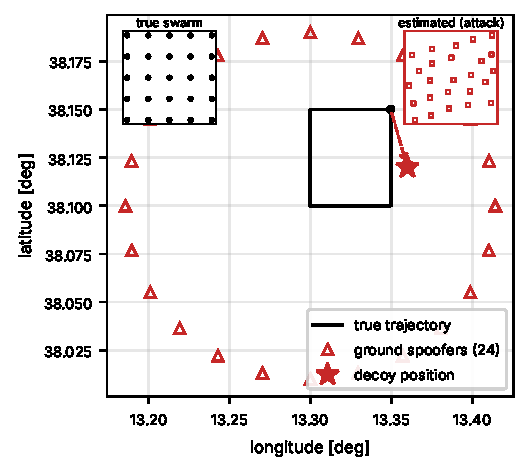
\includegraphics[width=\columnwidth]{fig_scenario}
\caption{Attack scenario (one epoch, $g=10$\,m). The swarm (true
positions, dots) flies its mission inside a 10\,km circle of 24 fixed
ground transmitters (triangles), each replaying one satellite. The
estimated fixes (open squares) are displaced onto the decoy (star) and
mildly dilated.}
\label{fig:scenario}
\end{figure}

\subsection{Attack effectiveness}
The attack succeeds: the centre UAV's estimated position is dragged by
the full decoy offset, 4.0\,km on average over the mission, at every
epoch (Fig.~\ref{fig:timeseries}, top), and every UAV in the swarm is
captured on all its visible satellites. The bottom panel shows the price
paid by a ground array: the relative-distance distortion is raised above
the no-attack noise floor throughout the mission.

\begin{figure}[!t]
\centering
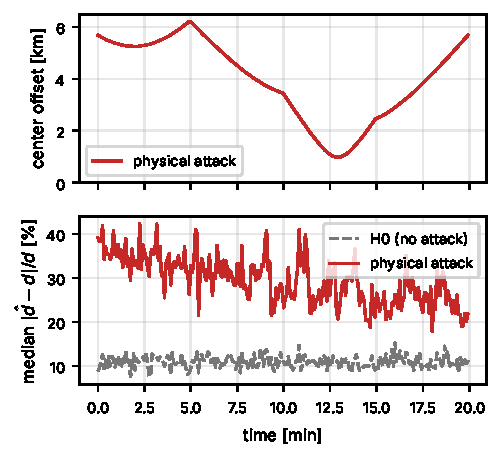
\includegraphics[width=\columnwidth]{fig_timeseries}
\caption{Per-epoch behaviour at $g=10$\,m (one mission). Top: position
offset of the centre UAV. Bottom: median relative-distance error with
and without the attack.}
\label{fig:timeseries}
\end{figure}

\subsection{Formation distortion and dilation}
Figure~\ref{fig:distortion} reports the median relative distance
distortion $E$ over the 20 missions (band: 10th--90th percentile across
missions). Under $H_0$ the distortion is pure GNSS noise and decays as
$1/g$, from 22\,\% at $g=5$\,m to 4.6\,\% at 20\,m. Under attack it
decreases from 38\,\% at 5\,m to 23\,\% at 20\,m, i.e.\ towards the
scale-free plateau of the residual~\eqref{eq:residual}, whose magnitude
depends on the elevations of the satellites in view and therefore varies
between missions. The sign of the residual is what
Remark~\ref{rem:collapse} predicts: the median distance ratio
$f_{\mathrm{maj}}=\operatorname{med}\,r_{ij}$ is $1.23$ under attack at
$g=20$\,m against $1.01$ without attack (and $1.37$ against $1.16$ at
5\,m, where noise biases both upward), and it exceeds one in every
attacked epoch. The computed formation is dilated by about a quarter of
the baseline; it never collapses.

\begin{figure}[!t]
\centering
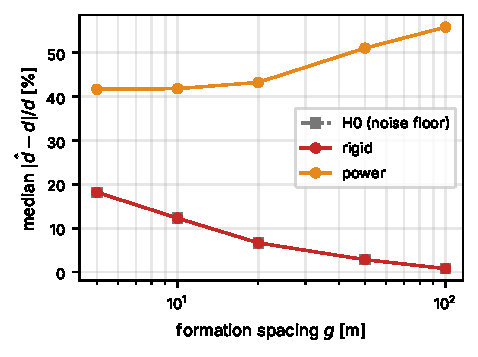
\includegraphics[width=0.92\columnwidth]{fig_distortion}
\caption{Median relative-distance distortion vs.\ formation spacing
(median over 20 missions; band: 10th--90th percentile across missions).}
\label{fig:distortion}
\end{figure}

\subsection{Detection performance}
Table~\ref{tab:pd} and Fig.~\ref{fig:pd} report $\PD$ at $\PFA=10^{-2}$
with 95\,\% confidence intervals, Table~\ref{tab:auc} the ROC areas, and
Fig.~\ref{fig:roc} the ROC curves at $g=10$\,m. Three observations
follow.

\begin{table*}[!t]
\caption{Detection probability at $\PFA=10^{-2}$ against the physical
distributed attack ($\sigma_{\mathrm{pr}}=3$\,m,
$\sigma_{\mathrm{rng}}=0.1$\,m; 20 missions, 4800 epochs per cell;
95\,\% CI from the paired mission bootstrap).}
\label{tab:pd}
\centering
\begin{tabular}{l cccc}
\toprule
$g$ [m] & Jansen min & Jansen max & Jansen majority & Consistency \\
\midrule
 5 & 0.005 [0.004, 0.011] & 0.007 [0.004, 0.009] & 0.000 [0.000, 0.000] & 0.029 [0.016, 0.048] \\
 8 & 0.002 [0.000, 0.004] & 0.003 [0.002, 0.005] & 0.000 [0.000, 0.000] & 0.065 [0.030, 0.117] \\
10 & 0.002 [0.000, 0.004] & 0.002 [0.001, 0.005] & 0.000 [0.000, 0.000] & 0.113 [0.039, 0.202] \\
12 & 0.001 [0.000, 0.004] & 0.001 [0.000, 0.003] & 0.000 [0.000, 0.000] & 0.153 [0.058, 0.264] \\
15 & 0.002 [0.000, 0.005] & 0.001 [0.000, 0.001] & 0.000 [0.000, 0.000] & 0.193 [0.085, 0.310] \\
20 & 0.001 [0.000, 0.003] & 0.000 [0.000, 0.001] & 0.000 [0.000, 0.000] & 0.262 [0.130, 0.423] \\
\bottomrule
\end{tabular}
\end{table*}

\begin{table}[!t]
\caption{ROC area (AUC) against the physical distributed attack; $0.5$
is chance, values below $0.5$ mean the attack moves the statistic away
from the alarm region.}
\label{tab:auc}
\centering
\begin{tabular}{l cccc}
\toprule
$g$ [m] & Jansen min & Jansen max & Jansen maj. & Consistency \\
\midrule
 5 & 0.312 & 0.430 & 0.171 & 0.570 \\
 8 & 0.262 & 0.378 & 0.072 & 0.622 \\
10 & 0.221 & 0.349 & 0.037 & 0.651 \\
12 & 0.189 & 0.324 & 0.019 & 0.676 \\
15 & 0.156 & 0.293 & 0.006 & 0.706 \\
20 & 0.122 & 0.255 & 0.001 & 0.743 \\
\bottomrule
\end{tabular}
\end{table}

First, \textbf{the collapse detectors are defeated at every spacing}:
all three Jansen variants give $\PD\le0.011$ (95\,\% upper bound), at or
below the false-alarm rate, and their AUC is \emph{below} chance---down
to $0.001$ for the majority variant at 20\,m, i.e.\ the attacked
statistic is larger than the authentic one in essentially every epoch.
This is the consequence of Remark~\ref{rem:collapse}: the distributed
attack dilates the formation, so the one-sided statistic
of~\eqref{eq:jansen} is pushed away from its threshold; the majority
variant, the one recommended in~\cite{jansen2016multireceiver}, never
fires at all. No threshold choice changes this.

Second, \textbf{the consistency test retains only marginal power}:
$\PD$ rises from $0.03$ at 5\,m to $0.26$ at 20\,m, with AUC from $0.57$
to $0.74$ and wide confidence intervals that reflect the
mission-to-mission variability of the residual. The test sees the
dilation only where it exceeds the $1/g$ noise floor of standard
positioning; over the whole formation-flight regime, three attacked
epochs out of four raise no alarm even at the widest spacing, and at
5--10\,m the attack passes essentially undetected.

Third, \textbf{the residual is the only handle the defender has}. It is
not a tuning artifact of the attack (power does not change it), it is
not removable by routing once the array encloses the operating area, and
it is the geometric cost of keeping the transmitters on the ground; its
magnitude is governed by the satellite elevations
through~\eqref{eq:residual}.

\begin{figure}[!t]
\centering
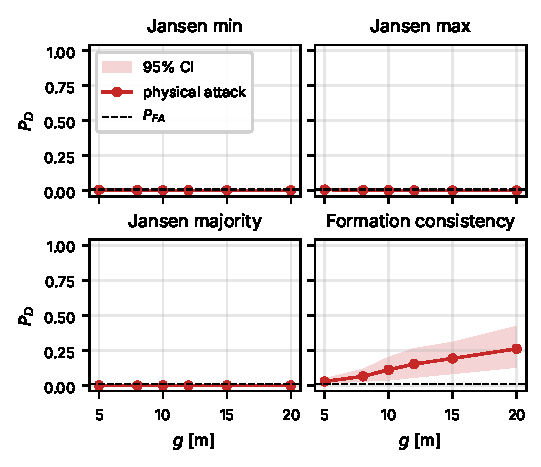
\includegraphics[width=\columnwidth]{fig_pd}
\caption{Detection probability vs.\ formation spacing at
$\PFA=10^{-2}$ for the four detectors (20 missions; band: 95\,\%
bootstrap CI). The collapse detectors never leave the $\PFA$ line.}
\label{fig:pd}
\end{figure}

\begin{figure}[!t]
\centering
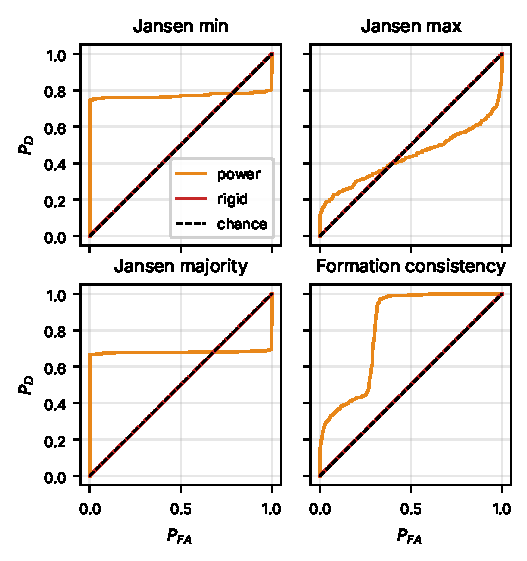
\includegraphics[width=\columnwidth]{fig_roc}
\caption{ROC curves at $g=10$\,m against the physical distributed
attack. The collapse detectors operate below chance.}
\label{fig:roc}
\end{figure}

% =========================================================================
\section{Discussion and Limitations}
\label{sec:discussion}

\subsubsection*{Scope of the result}
The evaluation covers detectors that are functions of relative
position/distance quantities---the collapse family and the two-sided
consistency family---over the spacing of GPS-based formation flight. The
former is blind for a structural reason (Remark~\ref{rem:collapse}) that
does not depend on the spacing; the latter is limited by the ratio
between the ground-array residual and the GNSS noise, and would detect
the attack for wide formations, for low-noise (RTK) fixes, or with
longer integration windows---our earlier runs at 50 and 100\,m gave
$\PD=0.56$ and $0.65$. The result does \emph{not} extend to
(i) \emph{direction-of-arrival} detectors: a circle of ground
transmitters produces arrivals at near-zero elevation, incongruent with
the satellite constellation, so multi-antenna arrays with attitude
information~\cite{psiaki2016gnss,borio2016sumofsquares} would see our
attacker, unless its transmitters are placed along the satellite
directions as in~\cite{tibaldo2025gnsswasp}; nor to (ii)
\emph{absolute-reference} checks---ranging to fixed infrastructure, TDoA
from ground sensor networks~\cite{jansen2018crowdgpssec}, terrain or
signal-of-opportunity positioning---for which the 4\,km displacement is
directly observable; nor to (iii) GNSS/INS detectors such as
SemperFi~\cite{sathaye2022semperfi} and INS innovation
monitors~\cite{tanil2018insmonitor,kujur2024insmonitor}, which respond to
the time variation of the induced error and were not evaluated.

\subsubsection*{Relation to formation-preserving attacks}
Tippenhauer et al.~\cite{tippenhauer2011requirements} prove that a
formation-preserving placement exists and
GNSS-WASP~\cite{tibaldo2025gnsswasp} realizes it with transmitters in
line with the satellites at altitude; Park and
Yoo~\cite{park2026rigidshift} show that an exactly common translation is
invisible to any relative-only detector. Our attacker is deliberately
more constrained, and the quantity we measure is what separates it from
those ideal attacks: a dilation of about 23\,\% of the baseline, enough
to be seen by a two-sided test on wide formations and too small to be
seen on the compact ones of formation flight. Raising the transmitters
would reduce the residual according to~\eqref{eq:residual}; we leave
that trade-off to future work.

\subsubsection*{Deployment and steady state}
The result assumes an array that encloses the swarm's operating area
(Section~\ref{sec:residual}); a static array that the swarm leaves
deforms the formation by more than 50\,\% and is readily detected. The
decoy position is constant, so the attack is modeled in its steady state
after capture; the transient at capture and time-varying decoys are not
modeled.

\subsubsection*{Other simplifications}
The simulator uses a spherical Earth, a synthetic constellation,
uncorrelated pseudorange noise (spatial correlation would lower the
detector's noise floor~\cite{jansen2016multireceiver} and favour the
consistency test), no multipath or shadowing, and signal capture by power
comparison without tracking-loop dynamics. Twenty missions per spacing
bound $\PD$ to within about $\pm0.1$ for the consistency test; the
conclusions on the collapse detectors do not depend on this resolution.

% =========================================================================
\section{Conclusion}
\label{sec:conclusion}
We evaluated the classical multi-receiver relative-distance spoofing
detectors against a physical distributed ground spoofer attacking a UAV
swarm in the 5--20\,m spacing of outdoor GPS-based formation flight,
simulating the attack transmitter by transmitter without any
idealization. The attack displaces the swarm by 4\,km and defeats the
collapse detectors of Jansen et al.\ in all their variants at every
spacing ($\PD\le0.011$, AUC below chance), because a distributed spoofer
dilates rather than collapses the computed formation and so never
produces the signature these detectors rely on. A two-sided consistency
check against independent UWB ranging retains only marginal power
($\PD$ from $0.03$ to $0.26$), limited by a residual dilation of about
23\,\% of the baseline that is the geometric cost of ground-based
transmitters and is masked by standard-GPS noise at these spacings.
Formation flight on GNSS therefore cannot rely on relative-distance
checks alone: they should be complemented by direction-of-arrival or
absolute-reference information, which the same residual analysis
identifies as the quantities a ground array cannot forge.

% =========================================================================
\section*{Acknowledgments}
\todo{ringraziamenti, funding}

\bibliographystyle{IEEEtran}
\bibliography{biblio}

\end{document}
